\documentclass[11pt]{article}
\usepackage[margin=0.7in]{geometry}
\usepackage{amsmath,amssymb,graphicx,xurl,hyperref,array}
\setlength{\parindent}{0pt}\setlength{\parskip}{4pt}
\setlength{\emergencystretch}{3em}
\begin{document}
{\Large Actual norm certificates to elliptic group relations}\par
2026-11-13. Source\path{6ba718256}. Unsigned evidence [pcc:unverified].

Let $K$ be a field, $W$ an actual Weierstrass curve with $a_1=a_3=0$,
and $f=X^3+a_2X^2+a_4X+a_6$. Let $S$ have distinct $x$ coordinates and
actual nonsingular points $P_x=(x,z(x))$. For $G=\prod_{x\in S}(X-x)$,
\[
 A(x)=z(x)B(x),\qquad A^2-fB^2=cG,\qquad c\ne0
 \quad\Longrightarrow\quad \sum_{x\in S}P_x=0.
\]
The final public theorem derives the certificate from singularity of the
actual barycentric signed Hankel matrix, for $|S|=2a$, $a\ge2$.
Neither a principal-ideal factorization nor a divisor/group relation is
assumed in that theorem [pcc:unverified].

\begin{center}
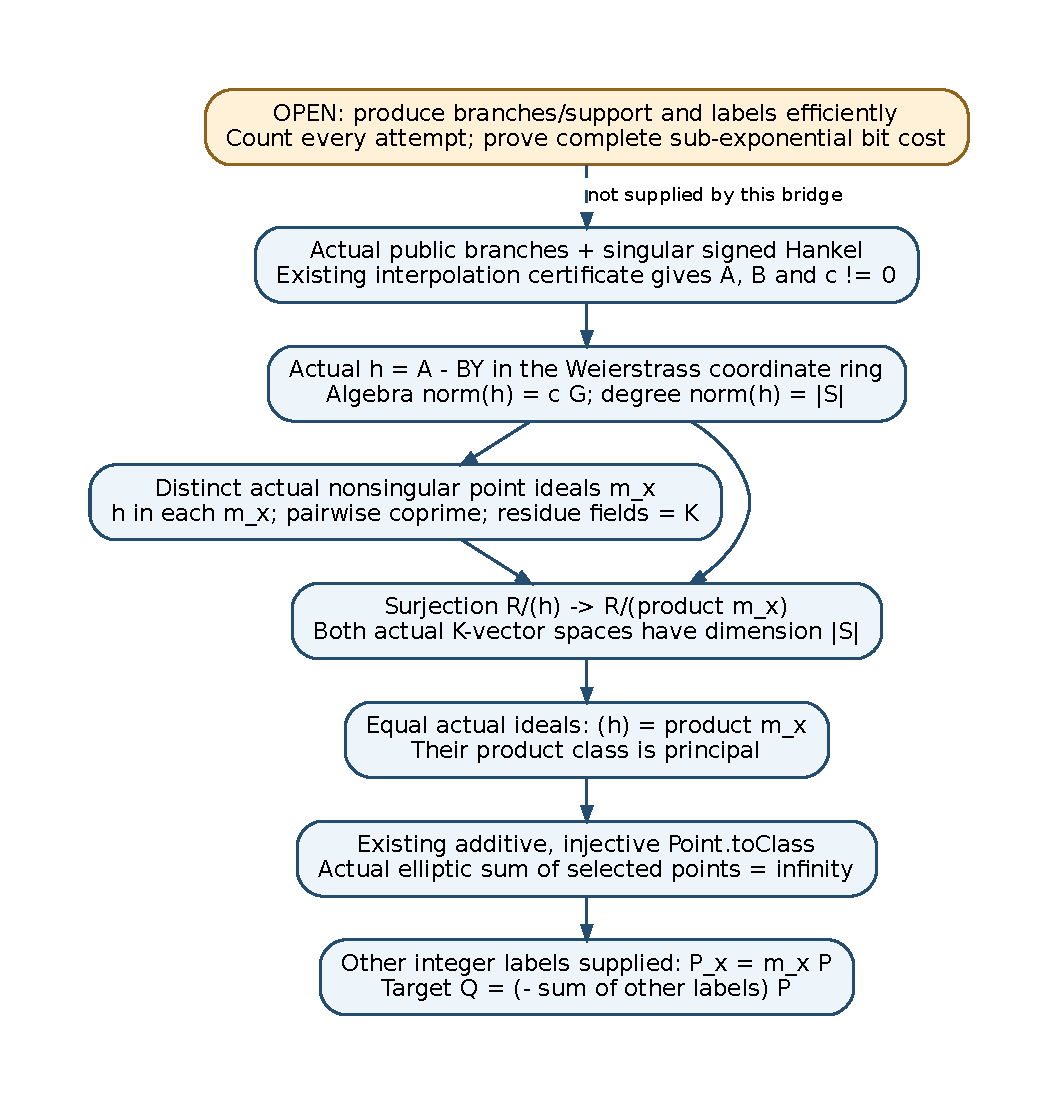
\includegraphics[width=0.94\linewidth,height=0.60\textheight,keepaspectratio]{bridge.pdf}
\end{center}

With all other integer labels supplied, $P_i=m_iP$ for $i\ne t$, the
actual target satisfies $Q=(-\sum_{i\ne t}m_i)P$. Its label is not a premise.
This certificate-to-group bridge does not produce the successful branches
or the other labels. See unsigned claims\path{PCC-20261113-c0da71} and
\path{PCC-20261113-3f21d1} [pcc:unverified].

\newpage
{\Large Actual-ring proof and fixed native controls}\par
\textbf{Proof.} Work in the actual ring $R=K[X,Y]/(W)$ with Mathlib's
rank-two $K[X]$ basis $(1,Y)$. For $h=A-BY$, its actual algebra norm is
$A^2-fB^2$. Each polynomial row gives $X-x\mid A-z(x)B$, so
$h\in\mathfrak m_x=(X-x,Y-z(x))$ by an explicit generator expression.
Distinct $x$ coordinates make these actual ideals coprime; their residue
fields are $K$. CRT gives $\dim_K R/(\prod\mathfrak m_x)=|S|$.
The nonzero principal quotient $R/(h)$ is finite dimensional through its
Smith-factor decomposition, and its dimension is $\deg\operatorname{Nm}(h)=|S|$.
The quotient map is surjective between equal finite dimensions, hence
injective, so $(h)=\prod\mathfrak m_x$. Its product class is principal.
The existing additive, injective Mathlib Point.toClass yields the actual
point sum. Separating the target summand gives the integer scalar relation
[pcc:unverified].

This reuses the established Angdinata--Xu ITP2023 ideal-class foundation,
sections3.1--3.3, rather than assuming a projective divisor library.
Nonsingularity is an explicit premise at every actual point. The field's
DecidableEq instance supports the library's point group. Repeated x
coordinates are outside the finite-set formulation. The original prime-field
objective retains its $p>3$ domain. No map to the earlier $W$-jet family
is assumed [pcc:unverified].

\textbf{Frozen controls.} The one native artifact uses $p=17$,
$f=X^3+2X+2$ and the following points, fixed prospectively:
\[(0,6),(3,1),(5,1),\quad(6,3),(10,11),(13,7).\]
\begin{center}\small
\begin{tabular}{p{0.40\linewidth}p{0.52\linewidth}}
Control & Recorded result\\\hline
Positive branches & All on curve, sum infinity, $\det M=0$\\
Full norm reconstruction & $A=[14,2,7,3]$, $B=[8,1]$, $c=9$; norm exactly $cG$\\
Flip only $(13,7)$ to $(13,10)$ & Sum$(10,6)=-2(13,7)$; $\det M=1$, kernel0\\
Base$(5,1)$, labels$[7,4,1,2,16,8]$ & Every supplied label matches by multiplication\\
Target fixed at node0 & Other labels sum31; $(-31)P=(0,6)$\\
Off-curve$(0,13)$; out-of-range inputs & Reject before group addition
\end{tabular}
\end{center}
Unsigned native claim\path{PCC-20261113-476fe0}. Artifact SHA256:\par
\path{3875f7bce92f789b273d026b3ea1aabada4eca4c559e92a65c9363f21432e0e5}.
JSON null means infinity. No order assertion or scalar search is used.
Unit tests reuse these fixtures; they are not independent yield trials
[pcc:unverified].

\textbf{Literal identity certificate.}
\path{IDC1hedd7e46a60a6ad5c} seals only the expansion
\[\det\left(\begin{smallmatrix}A&-FB\\-B&A\end{smallmatrix}\right)=A^2-FB^2.\]
The unchanged canonical native checker accepts32 statement-derived and16
extra replay points over its v1 fixed modulus. This does not interpret the
norm or execute Lean. Canonical hash/checker tests002 pass22; identity
clippy001 retains four existing style errors in unchanged canonical SHA256
under Rust1.99.1, without suppression. Separate main native14 tests and
strict clippy pass. All evidence remains unsigned [pcc:unverified].

\newpage
{\Large Formal statement map and exact evidence scope}\par
Lean4.35.0.\par
CryptoLean \path{148f5dc389b341401e06d76abe7783c4ccf42f2e}.\par
Mathlib \path{cfc55fc58714a59dc06e6e79edc6d1d95140d3c2}.\par
Module build010 and whole-study gate exit0:270 statements,0 additional
trusted axioms. Import-inclusive fresh replay session36245 exits0.
Each new statement uses only propext, Classical.choice and Quot.sound.
Default-PATH PCC checks remain source-only not\_covered, distinct from the
explicit toolchain checks; claims are unsigned [pcc:unverified].

\begin{center}\footnotesize
\begin{tabular}{p{0.34\linewidth}p{0.59\linewidth}}
NormGroupBridge declaration & Inputs and conclusion\\\hline
quotientFinite & Nonzero actual$h$; finite-dimensional$R/(h)$\\
idealsEqualOfDimension & Inclusion, both finite equal dimensions; actual ideal equality\\
pointIdealsCoprime & Distinct$x$; actual point ideals coprime\\
pointQuotientDimension & Injective$x$, actual nonsingular points; quotient dimension=count\\
principalPointProduct & Actual membership, nonzero$h$, exact norm degree; principal product\\
pointSumOfPrincipal & Actual nonsingular points, principal product; actual point sum0\\
normDegreePointSum & Derives that principal product from membership and norm degree\\
normFunctionNorm & $a_1=a_3=0$; actual algebra norm of actual$A-BY$\\
normFunctionAtPoint & Actual$A(x)=yB(x)$; actual point-ideal membership\\
fullNormPointSum & Rows, nonsingular points, norm$cG$, $c\ne0$; actual point sum0\\
cubicDegree & Actual cubic has degree3 for arbitrary lower coefficients\\
publicHankelPointSum & Exact cardinality, $a\ge2$, actual matrix determinant0; actual point sum0\\
targetScalarFromSum & Actual point sum0, other supplied labels; target integer\\
publicHankelTargetScalar & Composes actual public certificate, point sum and supplied-label scalar
\end{tabular}
\end{center}
The actual CRT/residue-field linear equivalence pointQuotientEquiv is
constructed within the dimension proof. Full normalized statement hashes,
source commit and17 unsigned claim records appear in
\path{group-bridge-evidence/claim-pins.json}; raw exits and source pins are in
\path{checks.json}, \path{fresh-status.json} and\path{source-inputs.sha256}.
Failed prototype001/002, module001--009 and identity attempts are preserved.
The identity tests001 include\_str failure preceded completion of sparse
hydration; after that file was confirmed, tests002 pass without source edits
[pcc:unverified].

\textbf{Sources checked.} KB MCP and executable wrapper are unavailable;
bounded fallback reads the pinned Mathlib Affine/Point, FreeModule/Norm,
IdealQuotient, Ideal operations/quotients and finite-dimensional APIs, plus
Angdinata--Xu ITP2023 sections3.1--3.3,
\url{https://doi.org/10.4230/LIPIcs.ITP.2023.6}.
Source-review receipt\path{sources-checked.json}, unsigned claim
\path{PCC-20261113-cee56b}. No novelty or exhaustive-survey claim
[pcc:unverified].

\textbf{Next obligation.} Produce actual branches/support and usable labels
with a constrained discrete finder, count every attempt and establish
complete expected bit cost. The original$\exp(o(\log r))$ acceptance criterion
is retained. This component supplies neither a visit bound nor a map from
the earlier$W$-base jet proposal. No performance graph, benchmark or leaderboard
value changes; this study's diagram and current problem record are updated
[pcc:unverified].
\end{document}
